\documentclass{beamer}

\usepackage[T1]{fontenc}       
\usepackage[utf8]{inputenc}    % pour les accents (mettre latin1 pour windows au lieu de utf8)
\usepackage[frenchb]{babel}    % le documents est en français
\usepackage{amsmath}           % un packages mathématiques
\usepackage{xcolor}            % pour définir plus de couleurs 
\usepackage{graphicx}          % pour insérer des figures
\usepackage{beamerthemesplit}

\setbeamercovered{transparent}
\usetheme[width=75pt,hideothersubsections]{Hannover}

\setbeamertemplate{headline}{\hskip 0.5cm \insertlogo }
\setbeamercolor*{titlelike}{parent=structure}

\useinnertheme{circles}
\setbeamertemplate{frametitle}[default][right]
\setbeamertemplate{blocks}[rounded][shadow=true]


%Title info
\title[OAR Cloud]{Une infrastructure légère de Cloud Computing basé sur OAR}
\logo{%
    
\includegraphics[width=1cm,height=0.5cm,keepaspectratio]{img/logo_pg2009.png}~%
    
\includegraphics[width=0.8cm,height=0.5cm,keepaspectratio]{img/logo_INRIA.png}%
}
\institute{Polytech Grenoble, INRIA\\\scalebox{2}{\insertlogo}}
\author{Michaël Mercier}
\date{2013}



% Faire apparaître un sommaire avant chaque section
\AtBeginSection[]{
   \begin{frame}
   \begin{center}{\Large Plan }\end{center}
   %%% affiche en début de chaque section, les noms de sections et
   %%% noms de sous-sections de la section en cours.
   \tableofcontents[currentsection, hideallsubsections]
   \end{frame} 
}
		

% Début de la présentation
% Contenu
\begin{document}
	% Page de titre
	\begin{frame}
		\titlepage
	\end{frame}
	
	
	% Sommaire
	\begin{frame} 
		\begin{center}{\Large Plan }\end{center}
		\tableofcontents[hidesubsections]
	\end{frame}
	
	
  \section{Projet OAR Cloud}
		\begin{frame}
			\frametitle{OAR Cloud}
			\begin{figure}
			  
\includegraphics[scale=0.3]{img/logo_oar.png}
 			\end{figure}
			Les objectifs du projet
			\begin{itemize}
			  \item Faire une définition plus précise du sujet
			  \item Etât de l'art
			  \item Tester les technologies émergentes
			  \item Identification des problèmes
			  \item Conception de l'architecture générale
			\end{itemize}			
		\end{frame}
			
			
			
	\section{Le Cloud omputing}
	
		\subsection{Définitions}
			\begin{frame}
			  \frametitle{Cloud computing}
			    \begin{block}{Wikipedia}
			      \textit{Le Cloud computing est l'accès via un réseau de télécommunications, à la demande et en libre-service, à des ressources informatiques partagées configurables}
			    \end{block}

			    Basé sur une pile de services
			    \begin{description}
			      \item[IaaS]\textit{ Infrastructure as a Service} 
			      Fournit un accès au ressources informatique simple et adaptable au besion
			      \item[PaaS]\textit{Platform as a Service}
			      Founit une plateforme pour faire tourné du code utilisateur
			      \item[SaaS]\textit{Software as a Service}
			      Fournit directement des applications
			    \end{description}
			\end{frame}
			
		\subsection{Outils}
			\begin{frame}
				\frametitle{Outils}
				OAR
				\begin{figure}
			    
\includegraphics[scale=0.3]{img/logo_oar.png}
 			  \end{figure}
 			  \begin{itemize}
   			  \item Gestionnaire de ressource informatique
   			  \item Dédié au HPC
   			  \item Stable et bien testé
   			  \item utilisé a grande echelle (Ex: Grid5000)
 			  \end{itemize}
			\end{frame}
	
		\subsection{Virtualisation système}
			\begin{frame}
			  \frametitle{Virtualisation système}
			  Différente solution basé sur les hyperviseurs à différents niveaux
			  \begin{columns}
          \begin{column}{.48\textwidth}
			      \begin{description}
			        \item[Type1] Directement sur le hardware
			      \end{description}
			    \end{column}%
          \hfill%
          \begin{column}{.48\textwidth}
            \begin{description}
			        \item[Type2] Au dessus de l'OS
			      \end{description}
          \end{column}
          \end{columns}
          \begin{figure}
			    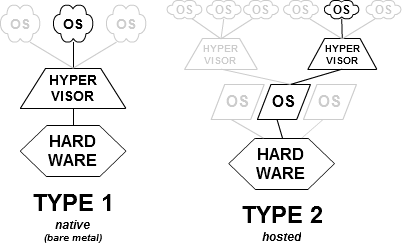
\includegraphics[scale=0.5]{img/Hyperviseur.png}
 			  \end{figure}
			\end{frame}
			
		\subsection{Outils}
			\begin{frame}
				\frametitle{LXC}
			\end{frame}
			
			
	\section{Virtualisation réseaux}
	
		\subsection{Définitions}
			\begin{frame}
			  \frametitle{Définitions}
			\end{frame}
			
		\subsection{Outils}
			\begin{frame}
				\frametitle{Outils}
			\end{frame}
			
			
	\section{Gestion de projet}
	
		\subsection{Journal}
			\begin{frame}
			  \frametitle{Journal}
			\end{frame}
			
		\subsection{Conception}
			\begin{frame}
				\frametitle{version 0.1}
			\end{frame}
			\begin{frame}
				\frametitle{version 0.3}
			\end{frame}
		
		\subsection{Organisation du travail}
			\begin{frame}
			  \frametitle{Organisation du travail}
			  \begin{itemize}
			    \item gestion d'équipe
			    \item contrainte du travail individuel
			  \end{itemize}
			\end{frame}
		
		
	\section{Bilans}
	  \begin{frame}
      \frametitle{Bilans}
		  \begin{itemize}
		    \item Bilan personnel
		    \item Bilan technique
		  \end{itemize}
	  \end{frame}
		
% 		\begin{alertblock}{}
% 		\end{alertblock}

% 		\begin{exampleblock}{ Points positifs }
% 		\end{exampleblock}
			
			
\end{document}
